\documentclass{article}%
\usepackage[T1]{fontenc}%
\usepackage[utf8]{inputenc}%
\usepackage{lmodern}%
\usepackage{textcomp}%
\usepackage{lastpage}%
\usepackage[head=40pt,margin=0.5in,bottom=0.6in]{geometry}%
\usepackage{graphicx}%
%
\title{\textbf{José Virtuoso: “La sociedad tiene que defender la Constitución”}}%
\author{EL NACIONAL WEB}%
\date{13/11/2018}%
%
\begin{document}%
\normalsize%
\maketitle%
\textbf{URL: }%
http://www.el{-}nacional.com/noticias/politica/jose{-}virtuoso{-}sociedad{-}tiene{-}que{-}defender{-}constitucion\_259602\newline%
%
\textbf{Periodico: }%
EN, %
ID: %
259602, %
Seccion: %
Política\newline%
%
\textbf{Palabras Claves: }%
NO\_TIENE\newline%
%
\textbf{Derecho: }%
12, %
Otros Derechos: %
CONTEXTO, %
Sub Derechos: %
\newline%
%
\textbf{EP: }%
NO\newline%
\newline%
%
\textbf{\textit{El rector de la Universidad Católica Andrés Bello considera que el Congreso Venezuela Libre debe promover la defensa de la Carta Magna de 1999 y construir entre todos los venezolanos una sociedad de dignidad y bienestar}}%
\newline%
\newline%
%
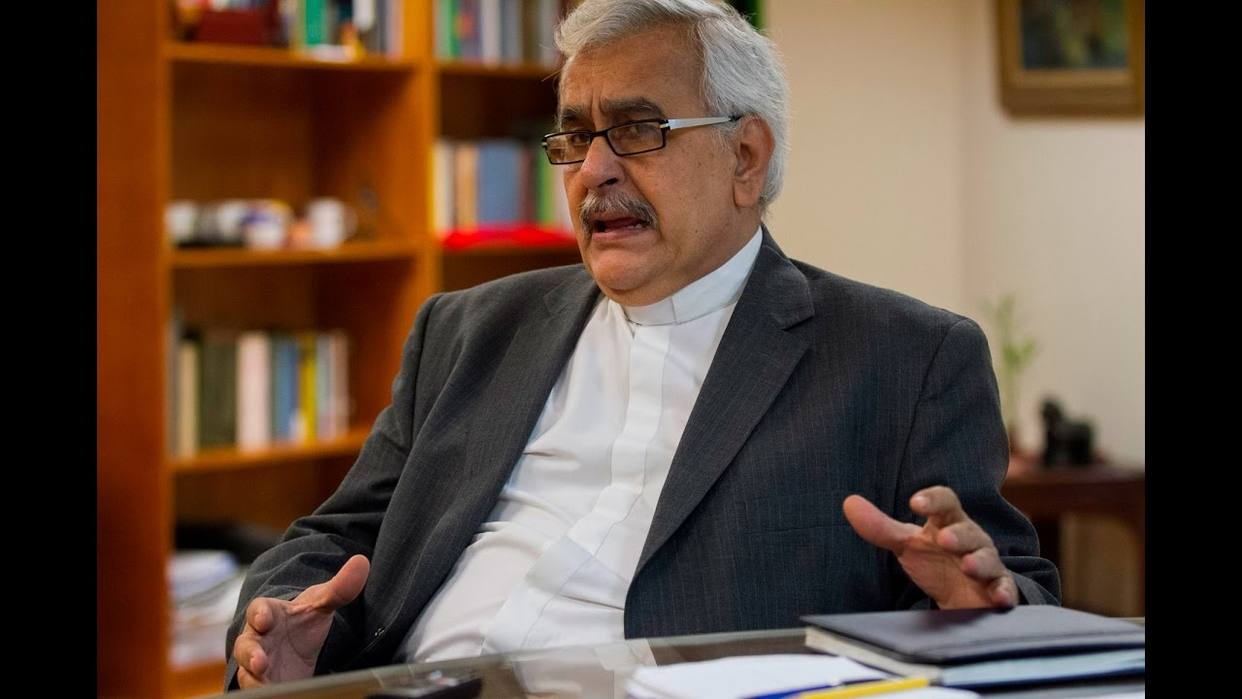
\includegraphics[width=300px]{66.jpg}%
\newline%
%
El rector de la Universidad Católica Andrés Bello (UCAB), José Virtuoso, advirtió que el país se acerca a una coyuntura muy peligrosa, debido a la proximidad del 10 de enero, fecha en la que de acuerdo con la Constitución finaliza el actual periodo del gobierno de Nicolás Maduro y debe asumir un nuevo presidente.%
\newline%
%
Resaltó que Venezuela no cuenta con un nuevo presidente electo porque el proceso del 20 de mayo fue calificado ilegítimo y fraudulento tanto por la Asamblea Nacional como por la comunidad internacional.%
\newline%
%
El sacerdote jesuita señaló que “ante esa prórroga no legítima de la actual presidencia de la República, la sociedad tiene que defender la Constitución vigente y su derecho a elegir cambiar sus gobernantes. La pregunta es qué vamos a hacer los venezolanos, precisamente para defender nuestros derechos”, aseguró el religioso.%
\newline%
%
Virtuoso destacó que el Congreso Venezuela Libre es un espacio importante para consensuar la defensa de la Carta Magna.%
\newline%
%
“En el corto plazo tiene una importancia clave: es el lugar donde todos los actores venezolanos podemos encontrarnos para defender el derecho a vivir en democracia, con libertad y justicia. Queremos convocar a todo nuestro pueblo para sentirnos como una gran fuerza, para construir esa sociedad de dignidad y bienestar que solo se puede lograr con democracia, participación y sobre todo cambio de las políticas públicas”, agregó el rector de la UCAB.%
\newline%
%
Virtuoso afirmó que para alcanzar la restitución del hilo democrático en el país, es necesaria la unidad de todos los sectores de la sociedad civil.%
\newline%
%
Con información de nota de prensa%
\newline%
%
\end{document}